
%(BEGIN_QUESTION)
% Copyright 2006, Tony R. Kuphaldt, released under the Creative Commons Attribution License (v 1.0)
% This means you may do almost anything with this work of mine, so long as you give me proper credit

A type ``S'' thermocouple is made of the dissimilar metals Platinum and Platinum-Rhodium (10\%) alloy.  Using a thermocouple table, determine the output voltages of a type ``S'' thermocouple at the following process temperatures:

$$\includegraphics[width=15.5cm]{i00369x01.eps}$$

\begin{itemize}
\item{} Voltmeter voltage = 11.857 mV; $T_{process}$ = ???$^{o}$ F 
\item{} Voltmeter voltage = 6.381 mV; $T_{process}$ = ???$^{o}$ F 
\item{} Voltmeter voltage = 1.972 mV; $T_{process}$ = ???$^{o}$ F 
\item{} Voltmeter voltage = 0 mV; $T_{process}$ = ???$^{o}$ F 
\end{itemize}

\vskip 10pt

Also determine the standard color codes for type S thermocouple wire:

\begin{itemize}
\item{} Positive conductor:
\item{} Negative conductor:
\item{} Thermocouple-grade jacket:
\item{} Extension-grade jacket:
\end{itemize}

\underbar{file i00369}
%(END_QUESTION)





%(BEGIN_ANSWER)

\begin{itemize}
\item{} Voltmeter voltage = 11.857 mV; $T_{process}$ = 2178$^{o}$ F 
\item{} Voltmeter voltage = 6.381 mV; $T_{process}$ = 1310$^{o}$ F 
\item{} Voltmeter voltage = 1.972 mV; $T_{process}$ = 502$^{o}$ F 
\item{} Voltmeter voltage = 0 mV; $T_{process}$ = 32$^{o}$ F 
\end{itemize}

\vskip 10pt

Color codes:

\begin{itemize}
\item{} Positive conductor: {\it Black} (extension grade -- no standard color for thermocouple grade)
\item{} Negative conductor: {\it Red} (extension grade -- no standard color for thermocouple grade)
\item{} Thermocouple-grade jacket: (no standard color for thermocouple grade)
\item{} Extension-grade jacket: {\it Green}
\end{itemize}

%(END_ANSWER)





%(BEGIN_NOTES)


%INDEX% Measurement, temperature: thermocouple (type S)

%(END_NOTES)


